\documentclass[11pt]{article}
\usepackage[T1]{fontenc}
\usepackage[utf8]{inputenc}
\usepackage[english]{babel}
\usepackage[normalem]{ulem}
\usepackage{amsmath}
\usepackage{xcolor}
\usepackage{listings}
\usepackage{listingsutf8}
\usepackage{lstautogobble}
\usepackage{titling}
\usepackage{fancyhdr}
\usepackage{graphicx}
\usepackage{underscore}
\usepackage{hyperref}
\usepackage{tabularx}
\graphicspath{{images/}}

\newcommand{\headerhaegri}{}
\newcommand{\headermidja}{University of Southern California}
\newcommand{\headervinstri}{}
\newcommand{\headerhaed}{14pt}
\newcommand{\headertykkt}{0.4pt}

% Title
\newcommand{\nafnanamskeidi}{CSCI531 Applied Cryptogrophy\\Final Project}
\newcommand{\nafnaverkefni}{EHR Audit System\\System Report}
\newcommand{\nafnanemanda}{Student: Hallgrimur David Egilsson\\USC ID: 6059-2639-79\vspace{4mm}}
\newcommand{\nafnakennara}{Professor: Dr. Tatyana Ryutov}
\newcommand{\dagsetning}{\today}
\setlength{\droptitle}{-20mm}
\newcommand{\haednemanda}{-2mm}
\newcommand{\haeddagsetningar}{0mm}
\newcommand{\haedtexta}{0mm}

% Page 1 footer
\newcommand{\footervinstri}{}
\newcommand{\footermidja}{}
\newcommand{\footerhaegri}{}
\newcommand{\footertykkt}{0.4pt}

% Page 2,3,4,... header
\lhead{CSCI 531}
\chead{}
\rhead{\nafnaverkefni}
\renewcommand{\headrulewidth}{0.4pt}

% Page 2,3,4,... footer
\lfoot{}
\cfoot{\thepage}
\rfoot{}
\renewcommand{\footrulewidth}{0.4pt}
\usepackage[top = 1.8in
   ,bottom=1.715in
   ,left=1.76in
   ,right=1.76in
   ]{geometry}


\let\oldfrac\frac
\let\frac\dfrac

\pagestyle{fancy}
\fancypagestyle{bls1}
{
	\fancyhf{}
	\lhead{\headervinstri}
	\chead{\headermidja}
	\rhead{\headerhaegri}
	\headheight = \headerhaed
	\lfoot{\footervinstri}
	\cfoot{\footermidja}
	\rfoot{\footerhaegri}
	\renewcommand{\headrulewidth}{\headertykkt}
	\renewcommand{\footrulewidth}{\footertykkt}
}

\title{
\huge\nafnanamskeidi\\
\vspace{8mm}
\nafnaverkefni\vspace{\haednemanda}}
\author{\nafnanemanda\\
        \nafnakennara\vspace{\haeddagsetningar}}
\date{\dagsetning\vspace{\haedtexta}}

\setlength{\parindent}{4em}
\setlength{\parskip}{4mm}

\renewcommand{\lstlistingname}{}
\lstset{frame=lines}
\lstset{caption={}}
\lstset{label={lst:code_direct}}
\lstset{basicstyle=\footnotesize}
\lstset{autogobble=true}
\lstset{literate = {-}{-}1}
\lstset{inputencoding=utf8/latin9}

\begin{document}
\maketitle
\thispagestyle{bls1}
	
\begin{flushleft}

\vspace{24mm}
I have read the Guide to Avoiding Plagiarism published by the student affairs office. I understand what is expected of me with respect to properly citing sources, and how to avoid representing the work of others as my own. The material in this paper was written by me, except for such material that is quoted or indented and properly cited to indicate the sources of the material. I understand that using the words of others, and simply tagging the sentence, paragraph, or section with a tag to the copied source does not constitute proper citation and that if such material is used verbatim or paraphrased it must be specifically conveyed (such as through the use of quotation marks or indentation) together with the citation. I further understand that overuse of properly cited quotations to avoid conveying the information in my own words, while it will not subject me to disciplinary action, does convey to the instructor that I do not understand the material enough to explain it in my own words, and will likely result in a lesser grade on the paper.

Signed: Hallgrimur David Egilsson

\newpage

\section{System architecture}

Figure \ref{fig:system_architecture} shows a high level overview of the main software components of the system.


\begin{figure}[h!]
\begin{center}
	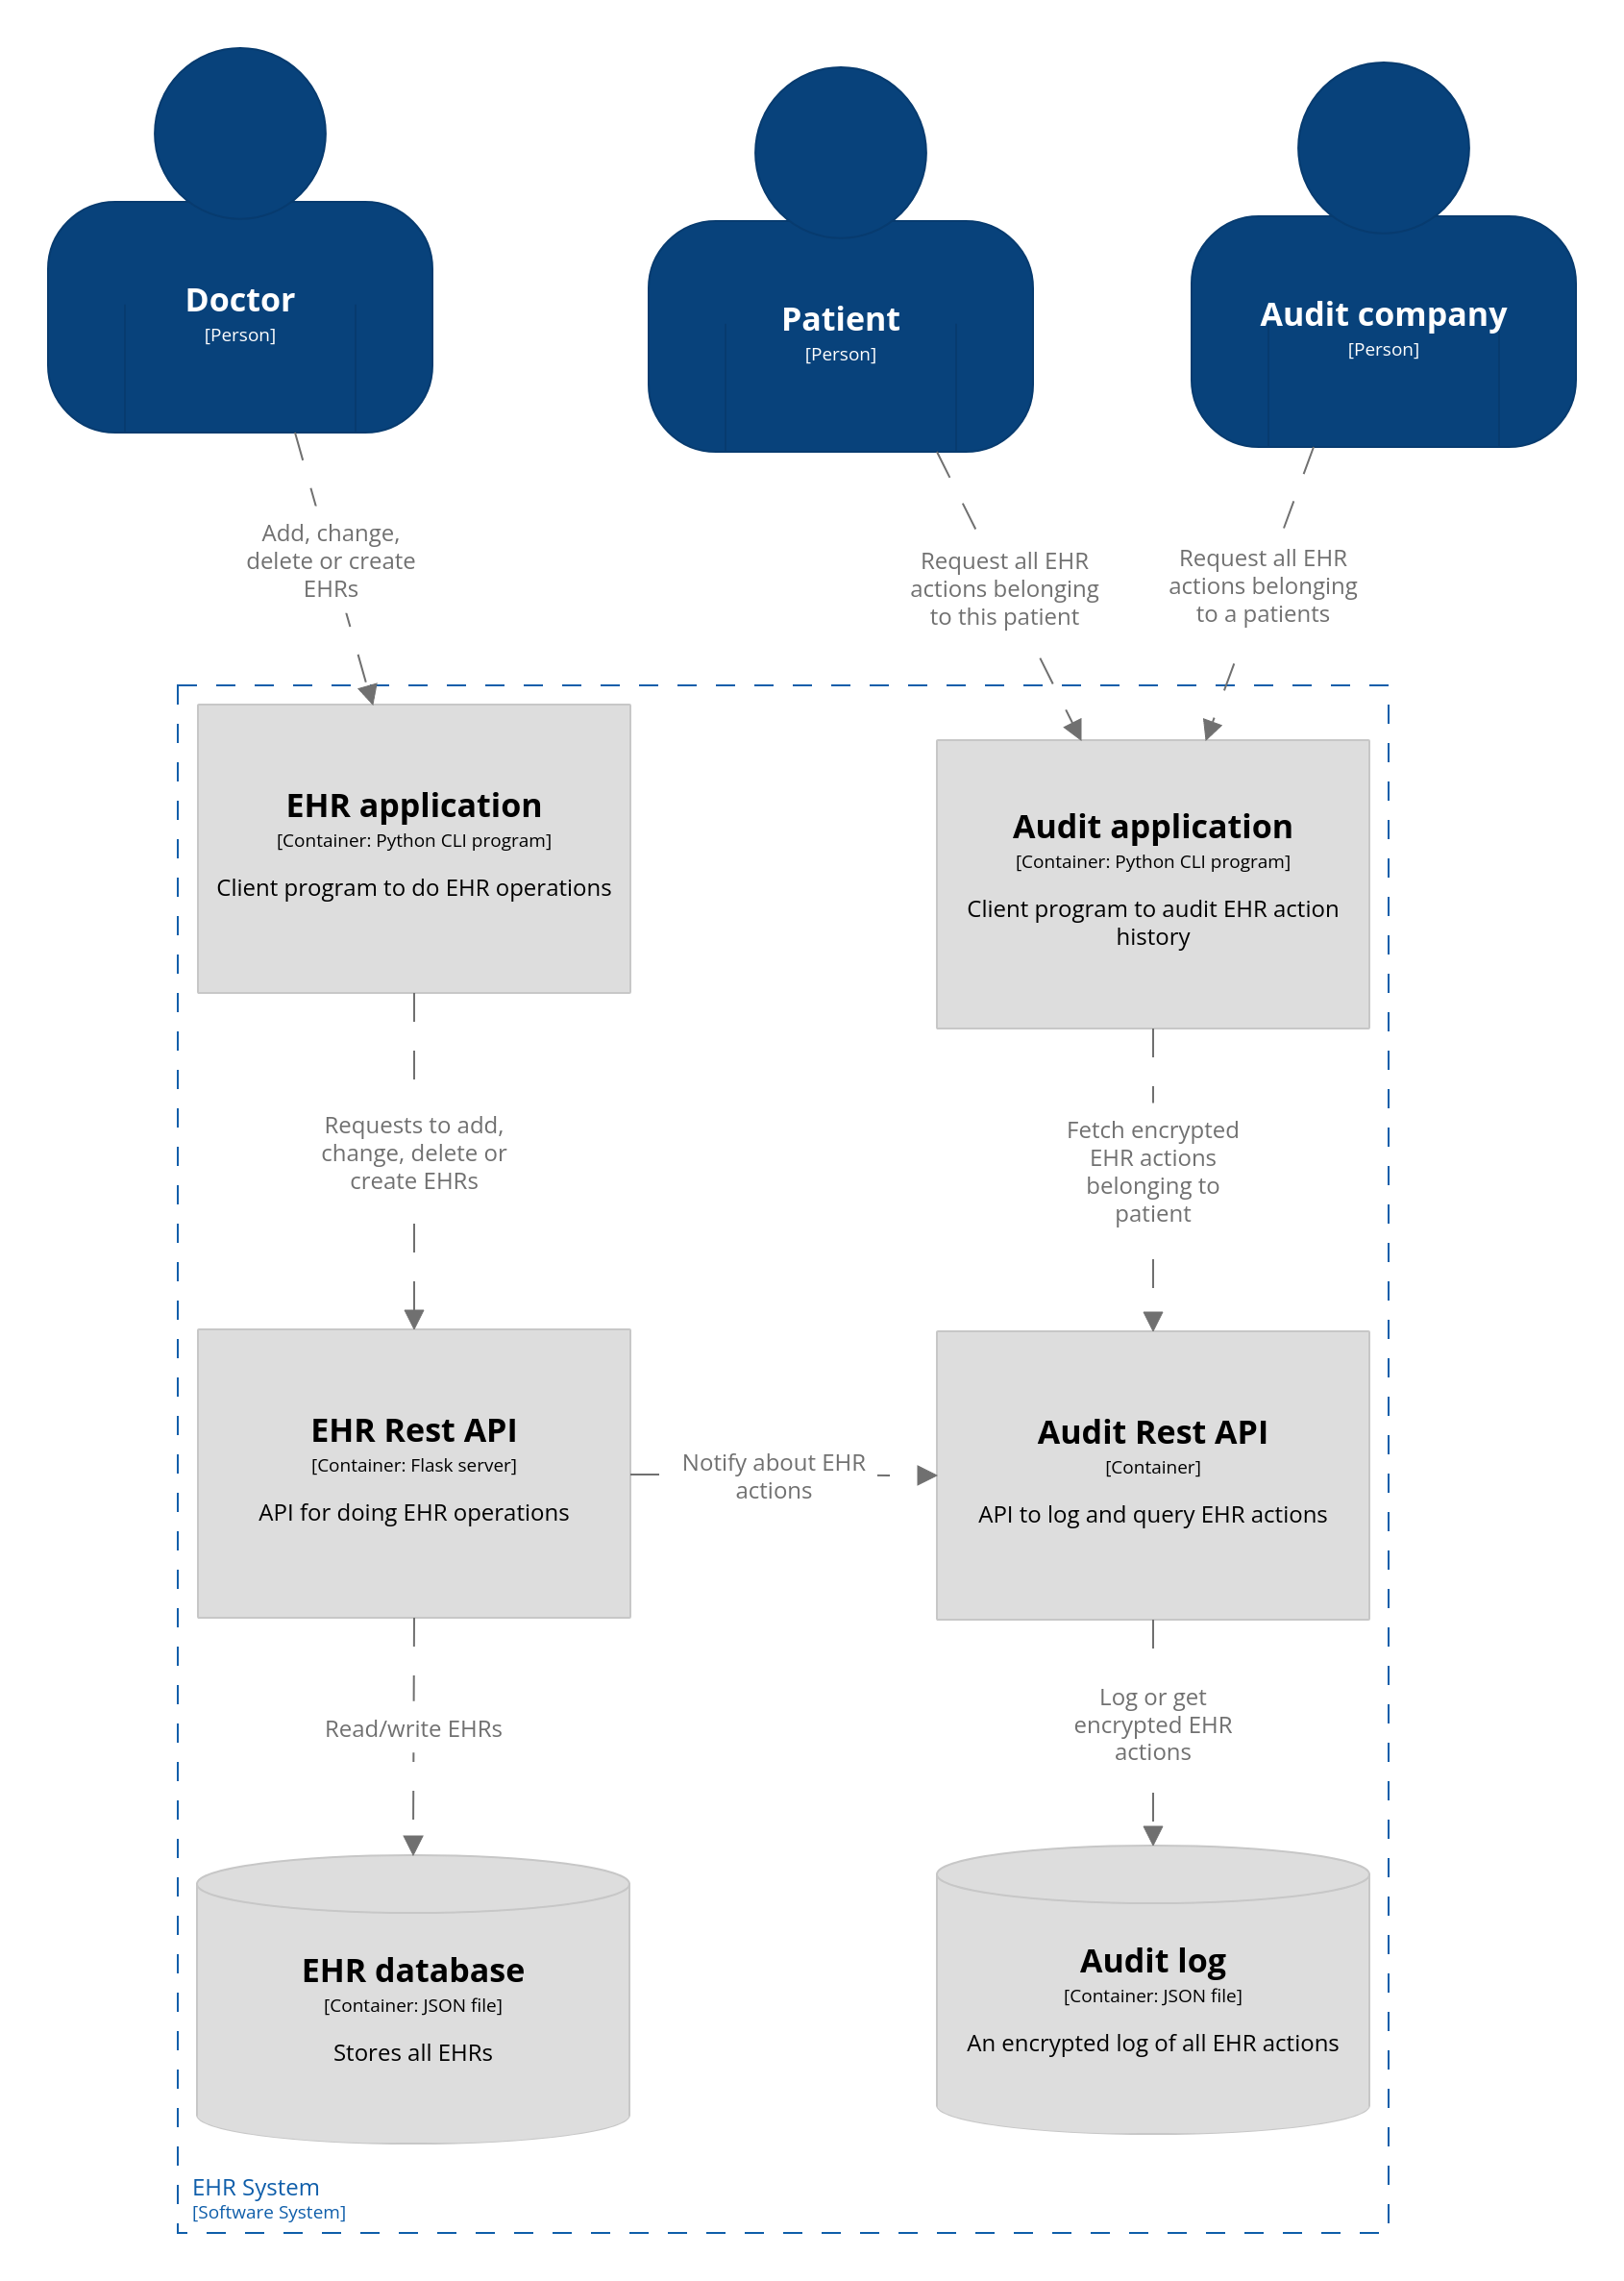
\includegraphics[width = 280px]{system_architecture_2.png}
	\caption{System overview}
	\label{fig:system_architecture}
\end{center}
\end{figure}

\newpage

First lets take a look at the EHR application, this is an application that only doctors should have access to which they can use during patient visits to modify EHRs (Electronic Health Records). The EHR application sends request to the EHR Rest API which handles reading and writing to the EHR database and notifying the Audit Rest API about EHR actions. Seperating the EHR application and the EHR Rest API allows the EHR application to be implemented with least priviledge, it should only be able to request actions on EHRs but not directly access the EHR database or independently call the Audit Rest API.

The Audit application is for patients and audit companies to read the EHR action history about a patient. The EHR action history of all patients is stored encrypted in the Audit log. Patients can only decrypt their own records in the audit log so direct access from the Audit application to the Audit log would not be too bad but still would leak some information, for example number of EHR actions in the log. Preferably the Audit application should only receive the patient's records which is what the Audit Rest API sends to the Audit application. The Audit application then proceeds to decrypt the patient's records and show them to the Audit application user.

Audit companies use the Audit application in the same way as a patient does but are authorized to fetch records for all patients registered under them.

\section{Cryptographic system architecture}

The overview in Figure \ref{fig:system_architecture} is a simplified view of the system because it does not show details like a Certificate Authority, system admin scripts, key storage and how the desired security goals are achieved. This chapter will explain the the cryptographic system architecture of the system.

Since the instructions for this project specified that the project should focus on the security of the audit log there were no security mechansisms designed or implemented for the EHR application, EHR Rest API or EHR database. In this project, these components are simply used to populate data in the audit log and to demonstrate the authorization mechansism in Audit Rest API which only allows the EHR Rest API to notify about EHR actions.

\subsection{Authentication and encryption in transit}

To be able to enforce authorization rules, clients connecting to Rest APIs must be authenticated, and to protect against attacks such as MitM or network sniffing, data in transit must be encrypted and integrity preserved.

In the design phase of this project it was explored to authenticate and encrypt messages using a similar design as in PGP \cite{pgpdesign}.

\begin{figure}[h!]
	\begin{center}
		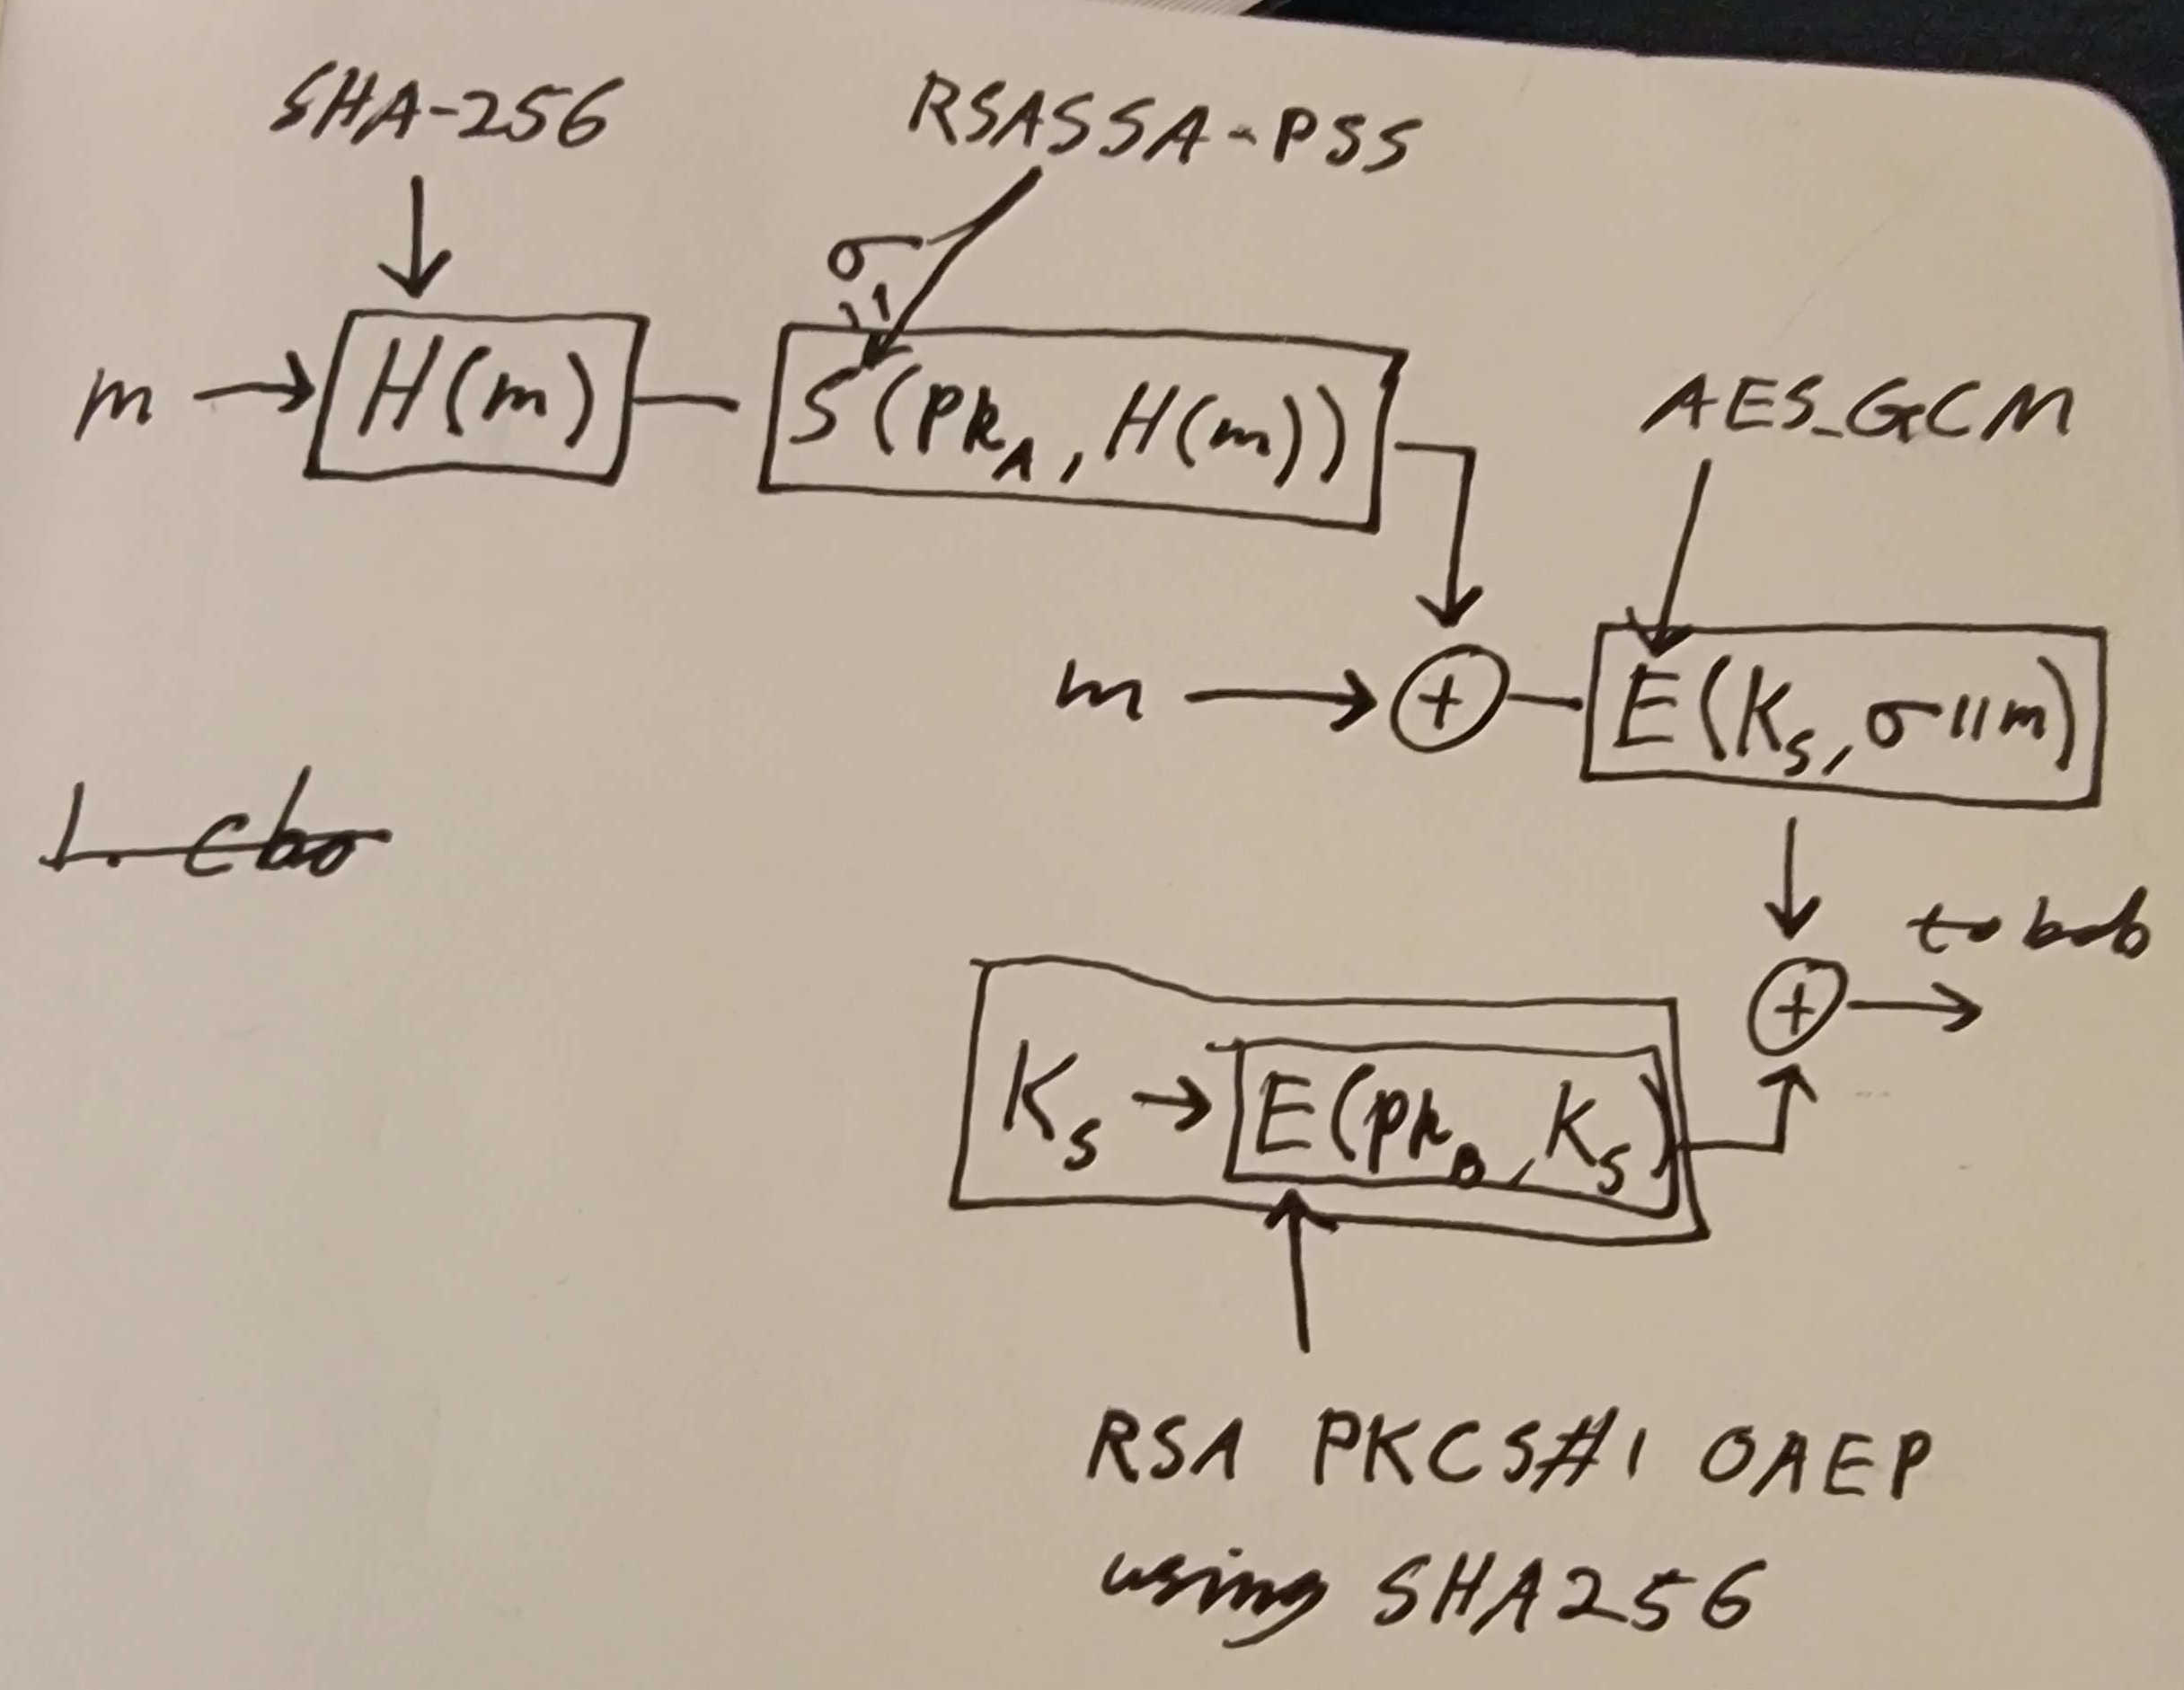
\includegraphics[width = 240px]{images/inspired_by_pgp_cropped.jpg}
		\caption{Initial design idea for authentication and encryption in transit}
		\label{fig:inspired_by_pgp}
	\end{center}
\end{figure}

Upon further inspection it was realized that there could be issues with this approach. For example, this design needs to be extended to protect against replay attacks. So at that point it was realized that there is a lot of room for error and mistakes in this design and it needed some rethinking.

Using TLS is a very common approach to solving the encryption-in-transit problem. On the web TLS is usually configured to authenticate only the server and afterwards the client is authenticated using password-based authentication at the application layer. Although not common on the web, the TLS protocol can be configured to do mutual authentication, which requires the client to hold a certificate as well as the server. Additionally it's designed to protect against attacks such as replay attacks \cite{TODO: find citation} which is an improvement from the previous design discussed.

Authenticating clients with TLS removes the need for implementing components needed for password-based authentication such as a database of salted and hashed passwords. However the TLS mutual authentication method requires the client to hold a certificate and a private key so connecting from multiple different devices becomes more difficult. Additionally the TLS solution requires a Certificate Authority to sign user certificates. It was anticipated that the client would need to hold more keys than the TLS keys so TLS with mutual authentication was picked to solve the authentication and encryption in transit problem.

\subsection{Encryption and integrity at rest}

Records in the audit log are encrypted at rest. The encryption needs to fulfill the following goals:

\begin{enumerate}
	\item For any given record in the database, only the patient the record belongs to, and the audit company of the patient, should be able to decrypt the EHR action included in the record.
	\item For any given record in the database, the Audit Rest API should be able to decrypt the patient's name in the record but not any other parts of it. This allows the Audit Rest API to find records for any given patient.
	\item Given access to the database, patients can discover which records belong to them but should not be able to discover the patient of other records, the same applies to Audit companies.
	\item If any record is tampered with, it should be detected and reported.
	\item If any record is deleted, it should be detected and reported.
	\item The database cannot be deleted by any single person or company.
\end{enumerate}

A record in the audit log is split into two parts: the patient's name and the EHR action.

The patient's name and the EHR action are encrypted using a hybrid cryptosystem \cite{TODO: add cite about what it is?}. The hybrid cryptosystem first generates a random 256-bit key and then encrypts the data using AES in Galois Counter Mode (GCM) which is a NIST recommendation for authenticated encryption \cite{TODO: add citation}. The GCM mode generates a tag that is stored along with the ciphertext which is used to detect tampering with the ciphertext or tag. The AES key is encrypted using RSA PKCS\#1 OAEP which requires a RSA public key. Remember that the database record is split into two parts, to encrypt the AES key to decrypt the patient's name, the Audit Rest API's RSA public key is used. The AES key to decrypt the EHR action is encrypted using two different RSA keys, one is the patient's public key and the other is the audit company's public key.

Although the AES ciphertext and tag are tamper-proof the encrypted RSA key is not, because RSA PKCS\#1 OAEP is not an authenticated encryption mechanism. So with the above design there is no protection against the encrypted AES key being tampered with. Therefore there was added one last step to the hybrid encryption mechanism: signing the encrypted AES key using RSASSA-PSS. The encrypted AES key is signed using a public RSA key of the Audit Rest API. To avoid using the same keys for RSA PKCS\#1 OAEP and RSASSA-PSS which could possibly decrease the overall security the system, the Audit Rest API holds two pairs of RSA keys, one set for encryption and decryption, the other set for signing and verifying.

The encryption mechanism described above protects against goals 1.-4. but does not fulfill goals 5. and 6. Although each record is tamper-proof there is no mechanism to detect if a record has been deleted as a whole. Additionally the database is centralized so whoever has access to the database, such as a system admin can delete it. Note that although it's possible to change the order of records in the database without detection it has no real effect since the plaintext of the EHR actions contain timestamps.

To achieve goal 6. the database must be decentralized and to achieve goal 5. there needs to be something that ties each record to the previous records. A blockchain cryptosystem would provide both of these features. For the blockchain to be truly decentralized the blockchain nodes cannot all be controlled by the same person or company. The blockchain will contain the records of the audit log which means that all parties controlling a blockchain node will learn the contents of the database. Since the records in the database are encrypted storing the database in a decentralized blockchain cryptosystem should not leak information about the contents of the EHR actions or its patients. However, if each record would be a block in the blockchain it would however leak information to the blockchain participants about how many EHR actions there are in the database and such as how fast they are growing. More generally, adversaries could perform traffic analysis on the data.

\subsection{Authorization rules}

Authorization is enforced in the Audit Rest API. The Audit Rest API requires all connecting clients to authenticate through TLS. For each call to the API endpoint the application layer reads the id of the connecting client from the TLS connection context and then uses the id to enforce authorization rules at the application layer.

The authorization rules enforced are as follows:

\begin{enumerate}
	\item Only the EHR Rest API is allowed to notify the Audit Rest API about EHR actions.
	\item A patient can only fetch encrypted EHR actions belonging to them.
	\item An audit company can only fetch encrypted EHR actions belonging to a patient that's registered under the audit company.
\end{enumerate}


\section{Implementation}

The project was implemented on a Ubuntu 21.04 machine but should run macOS as well. Since the project mostly relies on Python packages, getting it to run on Windows should not require a lot of changes either.

\subsection{IDs}

The user ID of the five users in the system are simply their names: \verb+alice+, \verb+bob+, \verb+carol+, \verb+david+, \verb+eve+. The server names have similar simple IDs: \verb+ehr_server+ and \verb+audit_server+ and finally the two audit companies have the IDs \verb+usc+ and \verb+ucla+.

\subsection{Audit company authorization rules}

It was decided that USC should be able to query the EHR action history of alice bob and eve. UCLA should be able to query the EHR action history of carol and david.

\subsection{The Network}

The project's proof of concept implementation runs on the local loopback interface. Although using networking was not a requirement of the project the benefits of doing it is that it helps keep component code organized, more similar to production systems and it makes using TLS is easier. Both the Rest APIs of the project only accept HTTPS connections and their TLS certificates bind their hostnames to their TLS public keys. Therefore therefor their domain names must be added to the local DNS. In linux this is possible by tying their domain names to the local loopback interface in \verb+/etc/hosts+:

\begin{figure}[h!]
	\begin{center}
		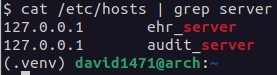
\includegraphics[width = 150px]{images/dns_config.png}
	\end{center}
\end{figure}

\verb+ehr_server+ was run on port 5000 and \verb+audit_server+ was run on port 5001.

\subsection{Applications, REST APIs and databases}

For simplicity the following technologies were chosen for each type of the software components:

\begin{tabularx}{0.8\textwidth} { 
		| >{\raggedright\arraybackslash}X 
		| >{\raggedright\arraybackslash}X | }
	\hline
	\textbf{Type} & \textbf{Technology} \\
	\hline
	Application  & Python CLI program  \\
	\hline
	REST API  & Python Flask server  \\
	\hline
	Database  & JSON file  \\
	\hline
\end{tabularx}

For TLS the Certificate Authority's keys are cert are stored in a \verb+system_admin+ folder in the implementation.

\subsection{Key generation}

The software components and users in the system all hold various private keys. For the project it was decided that they should be generated by a system admin and distributed to users and software components out of bounds.

\begin{figure}[h!]
	\begin{center}
		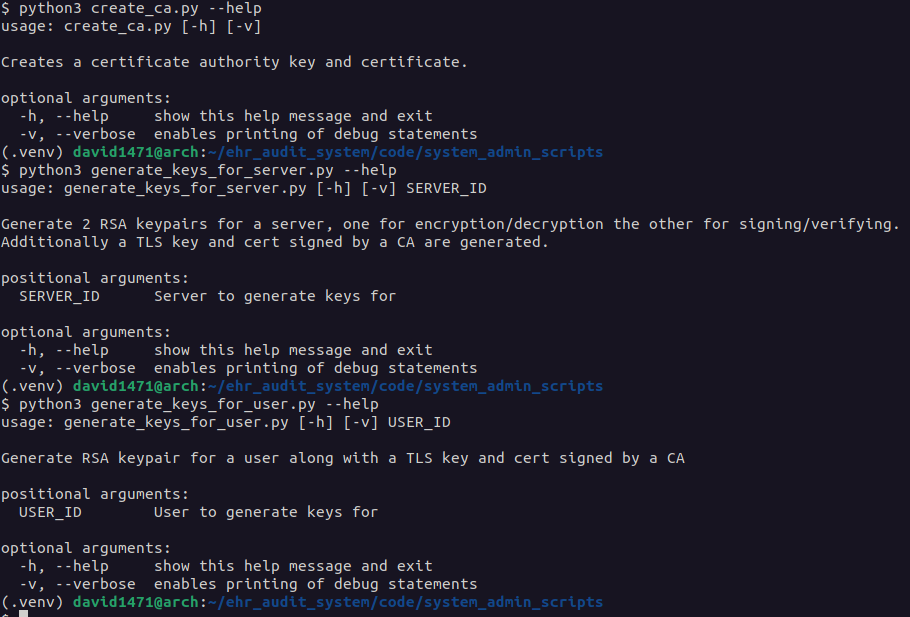
\includegraphics[width = 350px]{images/system_admin_scripts.png}
		\caption{Usage instructions of 3 system admin scripts implemented}
	\end{center}
\end{figure}

The key generation scripts depend on \verb+openssl+ being installed and on path. OpenSSL 'Version 1.1.1j  Feb 16 2021' was used in this project.

\subsection{TLS}

Audit server's Flask application was configured to use TLS and require mutual authentication:

\begin{figure}[h!]
	\begin{center}
		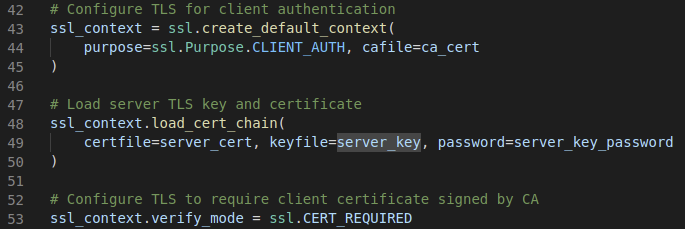
\includegraphics[width = 300px]{images/server_tls.png}
		
		\vspace{2mm}
		
		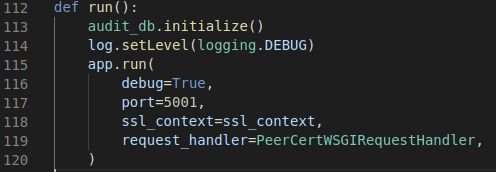
\includegraphics[width = 225px]{images/server_ssl_2.png}
		\caption{The TLS configuration for audit\_server}
	\end{center}
\end{figure}

To evade old and vulnerable versions of TLS it only accepts TLS 1.2 and TLS 1.3 connections. Preferably it should only accept TLS 1.3 connection but the easiest way to fix that would be to upgrade Python to version 3.10 which was decided to be out of scope for this project.


\begin{figure}[h!]
	\begin{center}
		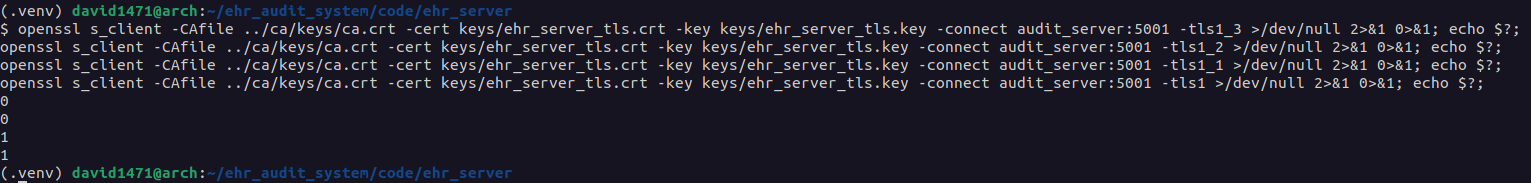
\includegraphics[width = 400px]{images/tls_version_verify.png}
		\caption{Verifying that the server only accepts TLS versions >= 1.2}
	\end{center}
\end{figure}

The TLS communications were also monitored through Wireshark as an exercise.

\subsection{The EHR application - generating data}
.

\begin{figure}[h!]
	\begin{center}
		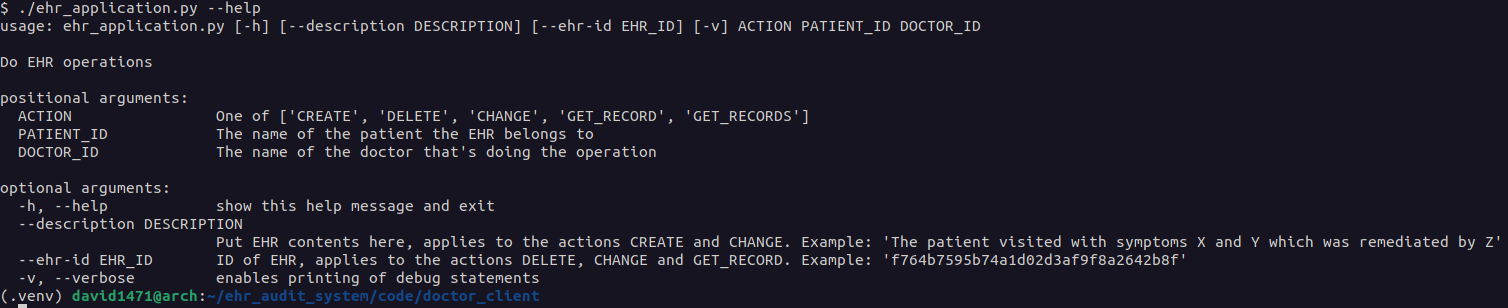
\includegraphics[width = 400px]{images/ehr_application_help.png}
		\caption{Usage instructions for the EHR application}
	\end{center}
\end{figure}

\begin{figure}[h!]
\begin{center}
	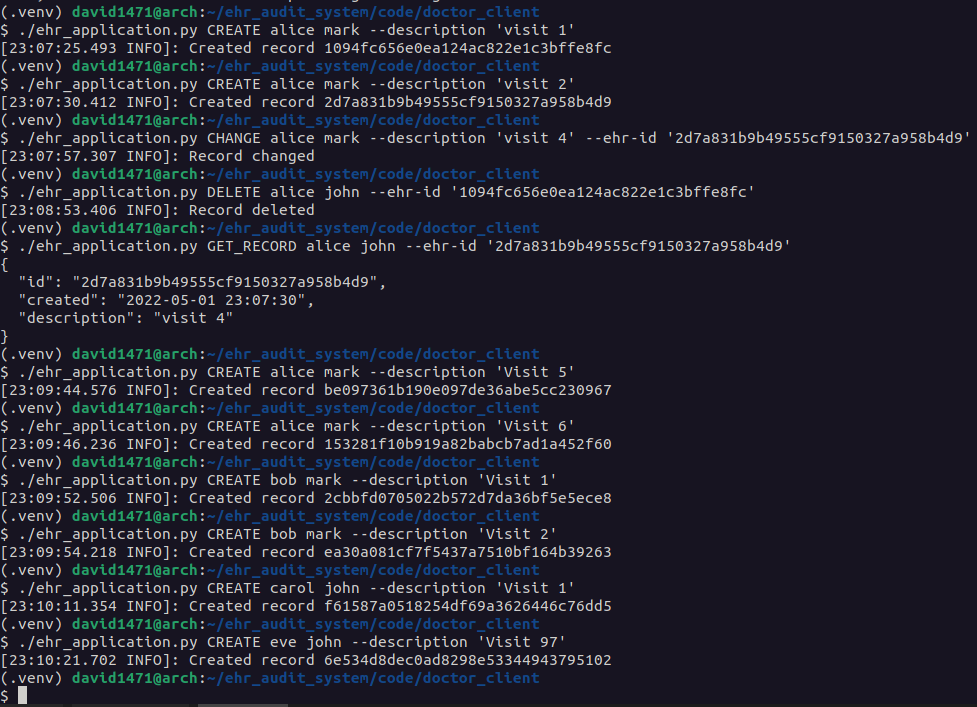
\includegraphics[width = 400px]{images/generating_data.png}
	\caption{Generating data using the EHR application}
\end{center}
\end{figure}

\begin{figure}[h!]
\begin{center}
	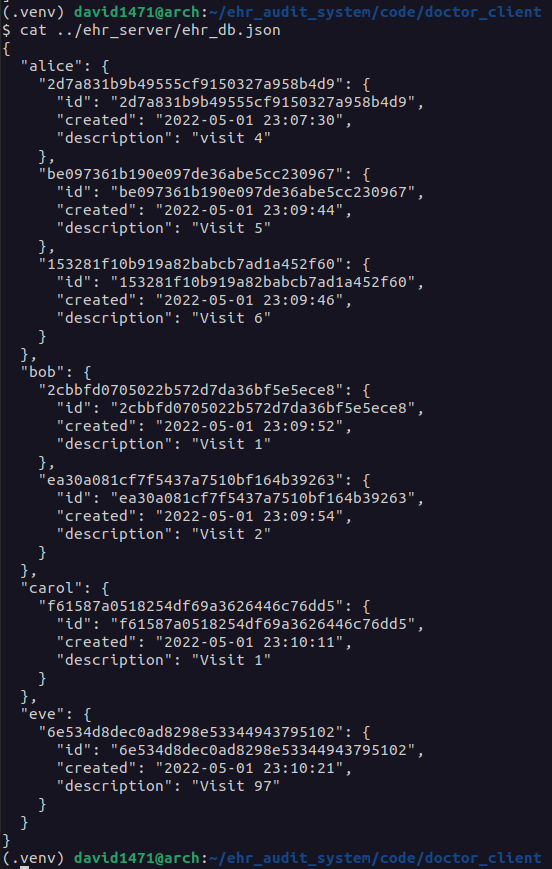
\includegraphics[width = 200px]{images/ehr_db_generated.png}
	\caption{The generated data in the EHR database.}
\end{center}
\end{figure}

.

\begin{figure}[h!]
\begin{center}
	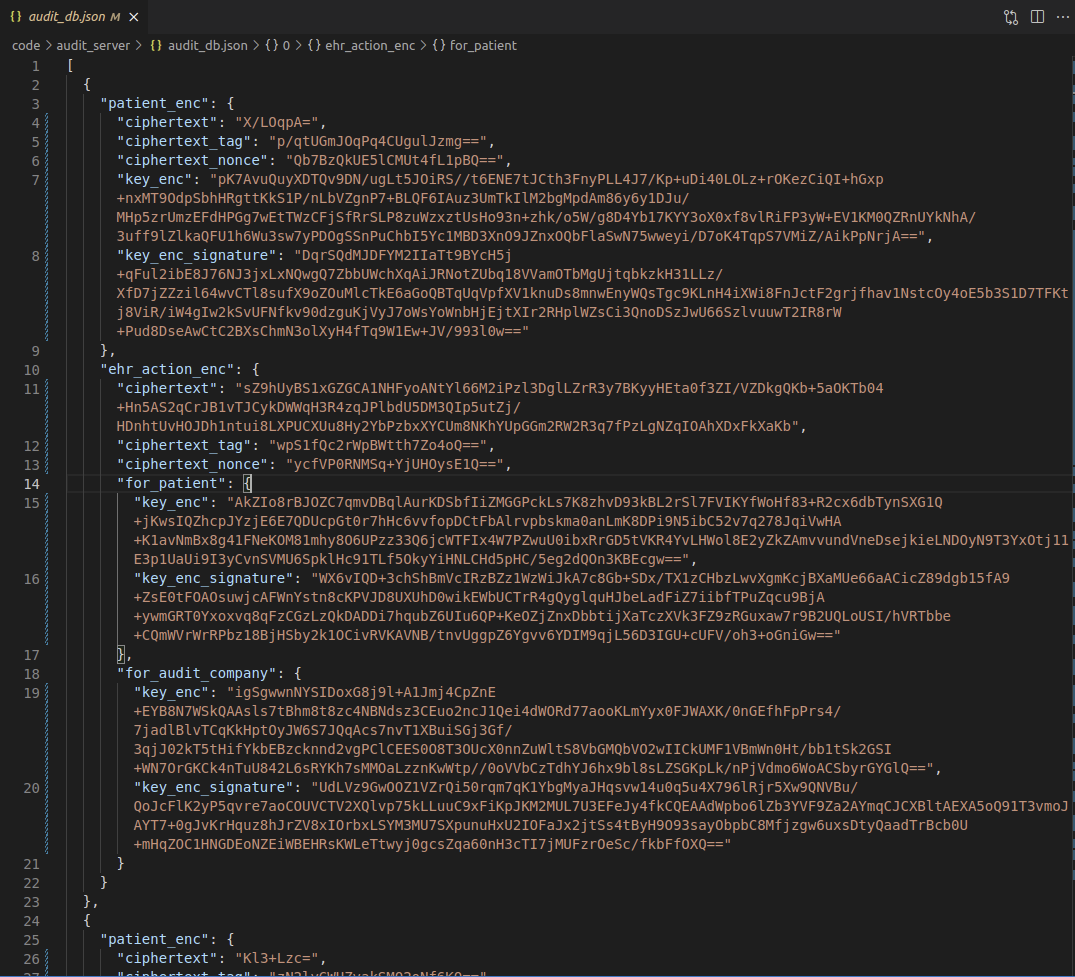
\includegraphics[width = 300px]{images/audit_db_enc.png}
	\caption{The first few lines of the audit log database}
\end{center}
\end{figure}

.

\subsection{The Audit log application - querying EHR action history}

\begin{figure}[h!]
	\begin{center}
		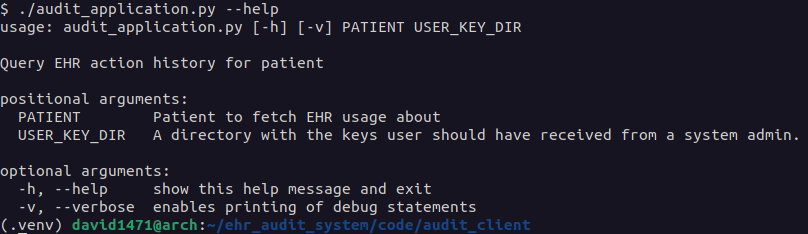
\includegraphics[width = 300px]{images/audit_application_help.png}
		\caption{Usage instructions for the Audit application}
	\end{center}
\end{figure}

\begin{figure}[h!]
\begin{center}
	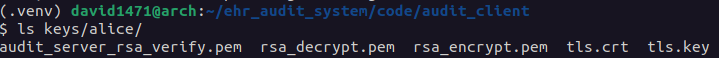
\includegraphics[width = 300px]{images/alice_keys.png}
	\caption{Alice's keys}
\end{center}
\end{figure}

\begin{figure}[h!]
\begin{center}
	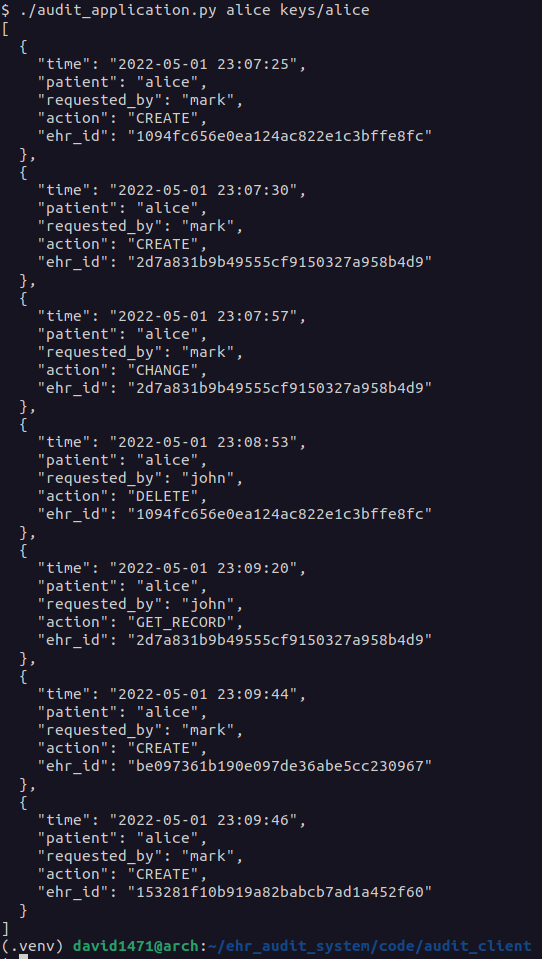
\includegraphics[width = 200px]{images/alice_history.png}
	\caption{Alice sucessfully fetching her EHR action history}
\end{center}
\end{figure}

\begin{figure}[h!]
\begin{center}
	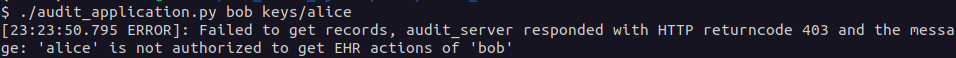
\includegraphics[width = 400px]{images/alice_fetch_error.png}
	\caption{Alice trying to fetch bob's history}
\end{center}
\end{figure}

\begin{figure}[h!]
\begin{center}
	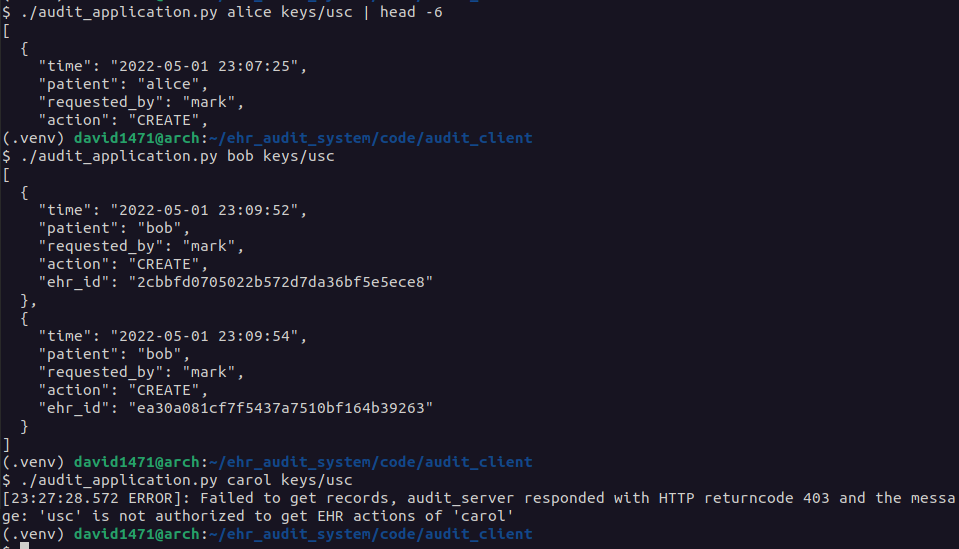
\includegraphics[width = 380px]{images/usc_fetch_requests.png}
	\caption{USC trying to fetch alice's, bob's and carol's EHR action history}
\end{center}
\end{figure}

\begin{figure}[h!]
\begin{center}
	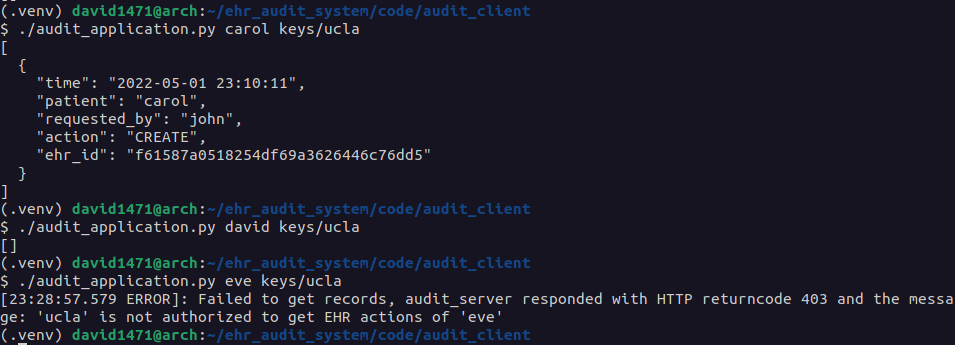
\includegraphics[width = 380px]{images/ucla_fetch_requests.png}
	\caption{UCLA trying to fetch carol's, david's and eve's EHR action history}
\end{center}
\end{figure}

\subsubsection{Fetching a record that has been tampered with}

Now one of the patient's name in the audit log database has been tampered with. It's detected once a user tries to fetch records:

\begin{figure}[h!]
	\begin{center}
		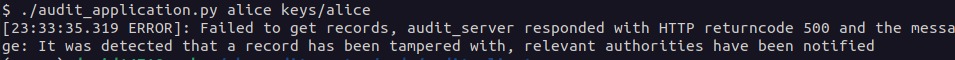
\includegraphics[width = 380px]{images/tamper_detection_server_side.png}
		\caption{Tamper detection server side}
	\end{center}
\end{figure}

Lets suppose the database has been restored again to its previous healthy state but now the EHR action part of one of alice's record has been tampered with, in this case the tamper detection happens client side (in the Audit application):

\begin{figure}[h!]
	\begin{center}
		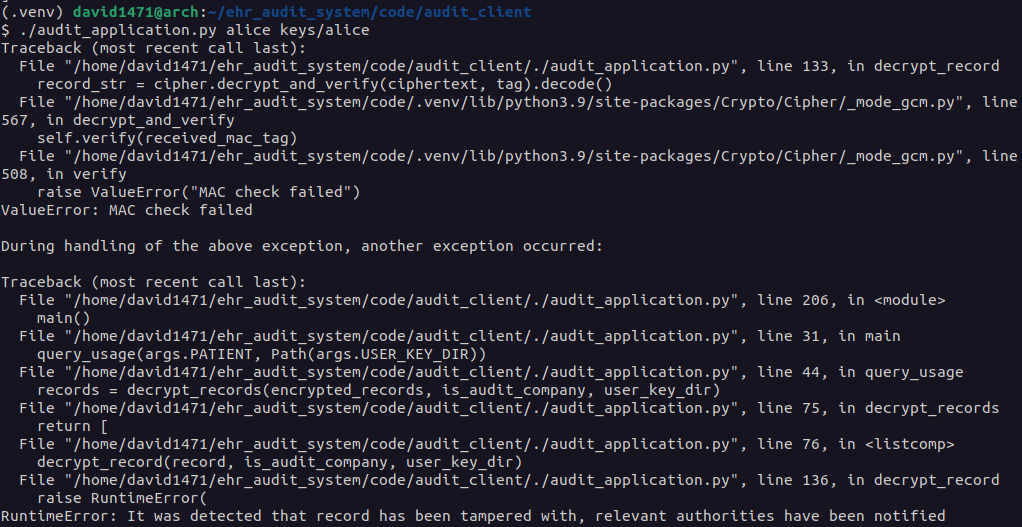
\includegraphics[width = 380px]{images/tamper_detection_client_side.png}
		\caption{Tamper detection client side}
	\end{center}
\end{figure}

\subsection{Encrypting database records}

To see the implementation of how the records are encrypted reading the code is the best way, but the idea was explained in the cryptographic system architecture chapter. The following image shows a record with comments explaining it parts.

\begin{figure}[h!]
	\begin{center}
		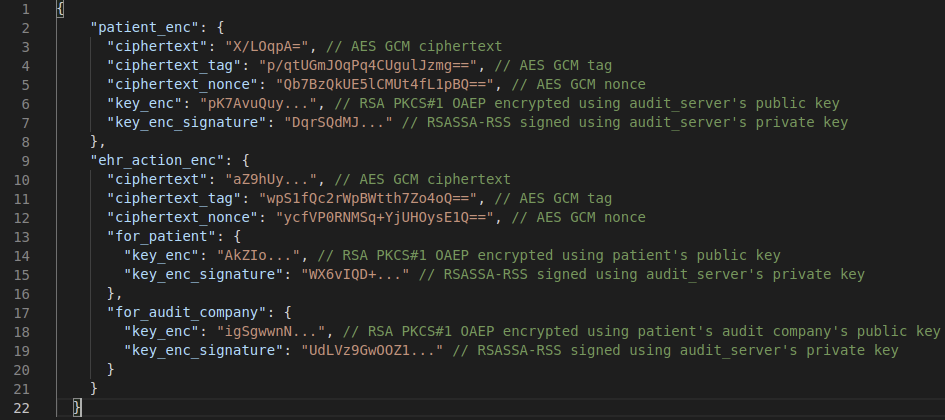
\includegraphics[width = 380px]{images/enc_record_parts.png}
		\caption{The parts of an encrypted record in the audit log database, some values shortened for the purpose of brevity.}
	\end{center}
\end{figure}

Looking at the encrypted patient names it was discovered that their length can leak information about who the patient is. Short names have short ciphertext entries and long names have long ciphertext entries. To fix this issue the ciphertext encrypt a SHA256 hash of the patient names instead of the names themselves. When the Audit server is looking up record it doesn't need to reverse the hash, it would compare the SHA256 hash of the patient its looking for with the results when the ciphertext is decrypted.







\newpage

\subsubsection{Notifying Audit Rest API about EHR actions}

.

\newpage


\subsubsection{Fetching encrypted EHR actions}




For simplicity of this PoC (Proof of Concept) the system will only support 5 hard-coded patients and 2 hard-coded audit companies. The patients in the systems will be:

Alice, Bob, Carol, David, Eve

The first audit company is USC and should be able to audit the EHR records of Alice, Bob and Eve.

The second audit company is UCLA and should be able to audit the EHR records of Carol and David.

Python pajsonckage setup follow recommendations at: https://packaging.python.org/en/latest/tutorials/packaging-projects/

EHR id generation:
* Explain the chance of generating two ids that are the same.

Database file:
* current: linux/ MAC OS lockin with /tmp/ehr_db.json

EHR REST API:
* POST data should always be in application/json

User IDs are just names for simplicity, we assume everyone has a uniqe name.

System architecture visualization: https://structurizr.com/dsl

Rest API specification: https://editor.swagger.io/

RSA PKCS\#1 OEAP max message length: \href{https://datatracker.ietf.org/doc/html/rfc8017#section-7.1}
	* Changed underlying hashing algorithm from SHA1 to SHA256 so max keysize is 190 bytes which is plenty enough (we just need 32 bytes for the 256 bit AES key)

Using different keys for encryption \& signing, probably more secure?

PEM key format:
*'PEM'*. (*Default*) Text encoding, done according to `RFC1421`_/`RFC1423`_.

The reason for timestamp is to make sure adversary can't do replay attack constantly and see how ciphertext grows (they might learn a visit to the doctor happened).

Instead of doing authentication inside the TLS channel, the TLS channel can be configured to use client keys as well, that would have been another option.

Authenticating clients: TLS client cert vs application level authentication
* TLS:
	* Built-in replay attack protection
	* Needs generation of certificates \& ngnix config
* Application level
	* Need to implement replay attack protection somehow (some timestamp shenanigans?)
	* More complex code

Better programming to do the TLS stuff in Ngnix and connect to Flask through Gunicorn or similar WSGI.

Name of doctor can be anything and is not verified, because it's not the focus of this project.

doctor client examples:

```
python3 ehr.py CREATE alice mark -d 'Visit 8'
python3 ehr.py DELETE alice john --ehr-id 73a6259260e4237019e1422c7b31adb0
python3 ehr.py CHANGE alice mark --description 'Visit 8' --ehr-id dee291db65e4cf73ca02c152468cc674
python3 ehr.py GET_RECORD alice john --ehr-id dee291db65e4cf73ca02c152468cc674
python3 ehr.py GET_RECORDS bob john
```

There is authorization check at https://audit_server:5001/log_action, only ehr_server can call it.
\begin{lstlisting}
```
curl -X POST --cacert ca/keys/ca.crt --cert audit_client/keys/bob/tls.crt --key audit_client/keys/bob/tls.key https://audit_server:5001/log_action
bob is not authorized to log EHR actions(.venv) david1471@arch:~/ehr_audit_system/code
curl -X POST --cacert ca/keys/ca.crt --cert audit_client/keys/bob/tls.crt --key audit_client/keys/bob/tls.key https://audit_server:5001/log_action
bob is not authorized to log EHR actions
(.venv) david1471@arch:~/ehr_audit_system/code
curl -X POST --cacert ca/keys/ca.crt --cert ehr_server/keys/ehr_server_tls.crt --key ehr_server/keys/ehr_server_tls.key https://audit_server:5001/log_action
<!doctype html>
<html lang=en>
<title>400 Bad Request</title>
<h1>Bad Request</h1>
<p>Did not attempt to load JSON data because the request Content-Type was not &#x27;application/json&#x27;.</p>
```
\end{lstlisting}

Username can't be to long, otherwise RSA PKCS\#1 OAEP breaks because encrypted message will become to large

System admin commands:
\begin{lstlisting}
```
for user in alice bob carol david eve usc ucla; do cp audit_client/keys/${user}/rsa_encrypt.pem audit_server/keys/known_pubkeys/${user}/
```
\end{lstlisting}

Possible vulnerability: determine patient name length on length of ciphertext

Possible vulnerability: there is no protection against swapping ehr_action_enc in the database, impact not great because of encryption.

\section{Introduction}

\section{System architecture}

\textit{Describe the system components (e.g., authentication server, audit server, etc.), their functionality, and communication patterns. Clearly describe how your system meets the five goals discussed above.}

\section{Cryptographic components}

\textit{discuss appropriate choice of specific cryptographic primitives to ensure the system supports the goals outlined above.}

\textit{Describe the concrete encryption schemes and key management approaches to be used in your system}

\section{Limitations of the system}

\textit{Which challenges were not addressed?}

\section{Example section}

Example citation \cite{neuman2009challenges}

\subsection{Example subsection 1}

\subsection{Example subsection 2}

\newpage

\bibliography{citations.bib}

\bibliographystyle{ieeetr}


\end{flushleft}
	
\end{document}
